\section{The Extension of Our Model}
\label{sec_extension}
In this section, we extend our model to consider other factors (\eg. time evolution) and discuss how those factors influence our model.

\subsection{The Time Evolution of Charging Station Construction}
\label{time}
When considering the time evolution of the charging station construction, a competition model based on Voltera Equation has been applied. Where the competition relation is given by,

\begin{equation}
\label{competition}
  \frac{d}{dt} N_i = r_i x_i ( 1- \frac{\sum \alpha_{ij}x_j}{K_i})
\end{equation}
Where $N_i$ is the number of a certain specie, $\alpha$ is a second order tensor describing the iteration among different "species". When there are 2 "species", which can be reasonable determined through historical data.

For our case, the problem is reduced to a 2 "species" competing problem. Where we set $N_e,N_t$ as the number of electrical vehicles and traditional vehicles respectively.

Therefore the Lotka-Volterra equations are:

\begin{equation}
\label{competition_2}
\left\{
       \begin{array}{lr}
             \frac{d}{dt} N_e & = r_e N_e ( 1- \frac{N_e+\alpha_{12}N_t}{K_1})\\
             \frac{d}{dt} N_t & = r_t N_t ( 1- \frac{N_t+\alpha_{12}N_e}{K_2})
       \end{array}
\right.
\end{equation}



For simplicity, we assume that the total capacity of charging stations is proportional to the number of electrical vehicles $N_e$, i.e.

\begin{equation}
\label{propor}
  \sum Cap(i) \varpropto N_e
\end{equation}

Which indicates that the construction of charing station can be guided by the time evolution of electric vehicles.

For the case in Ireland, we can predict the evolution process based on Equation~\ref{competition_2}, \
and Figure~\ref{fig_evolution} show the result of our prediction.
\begin{figure}[!t]
\centering
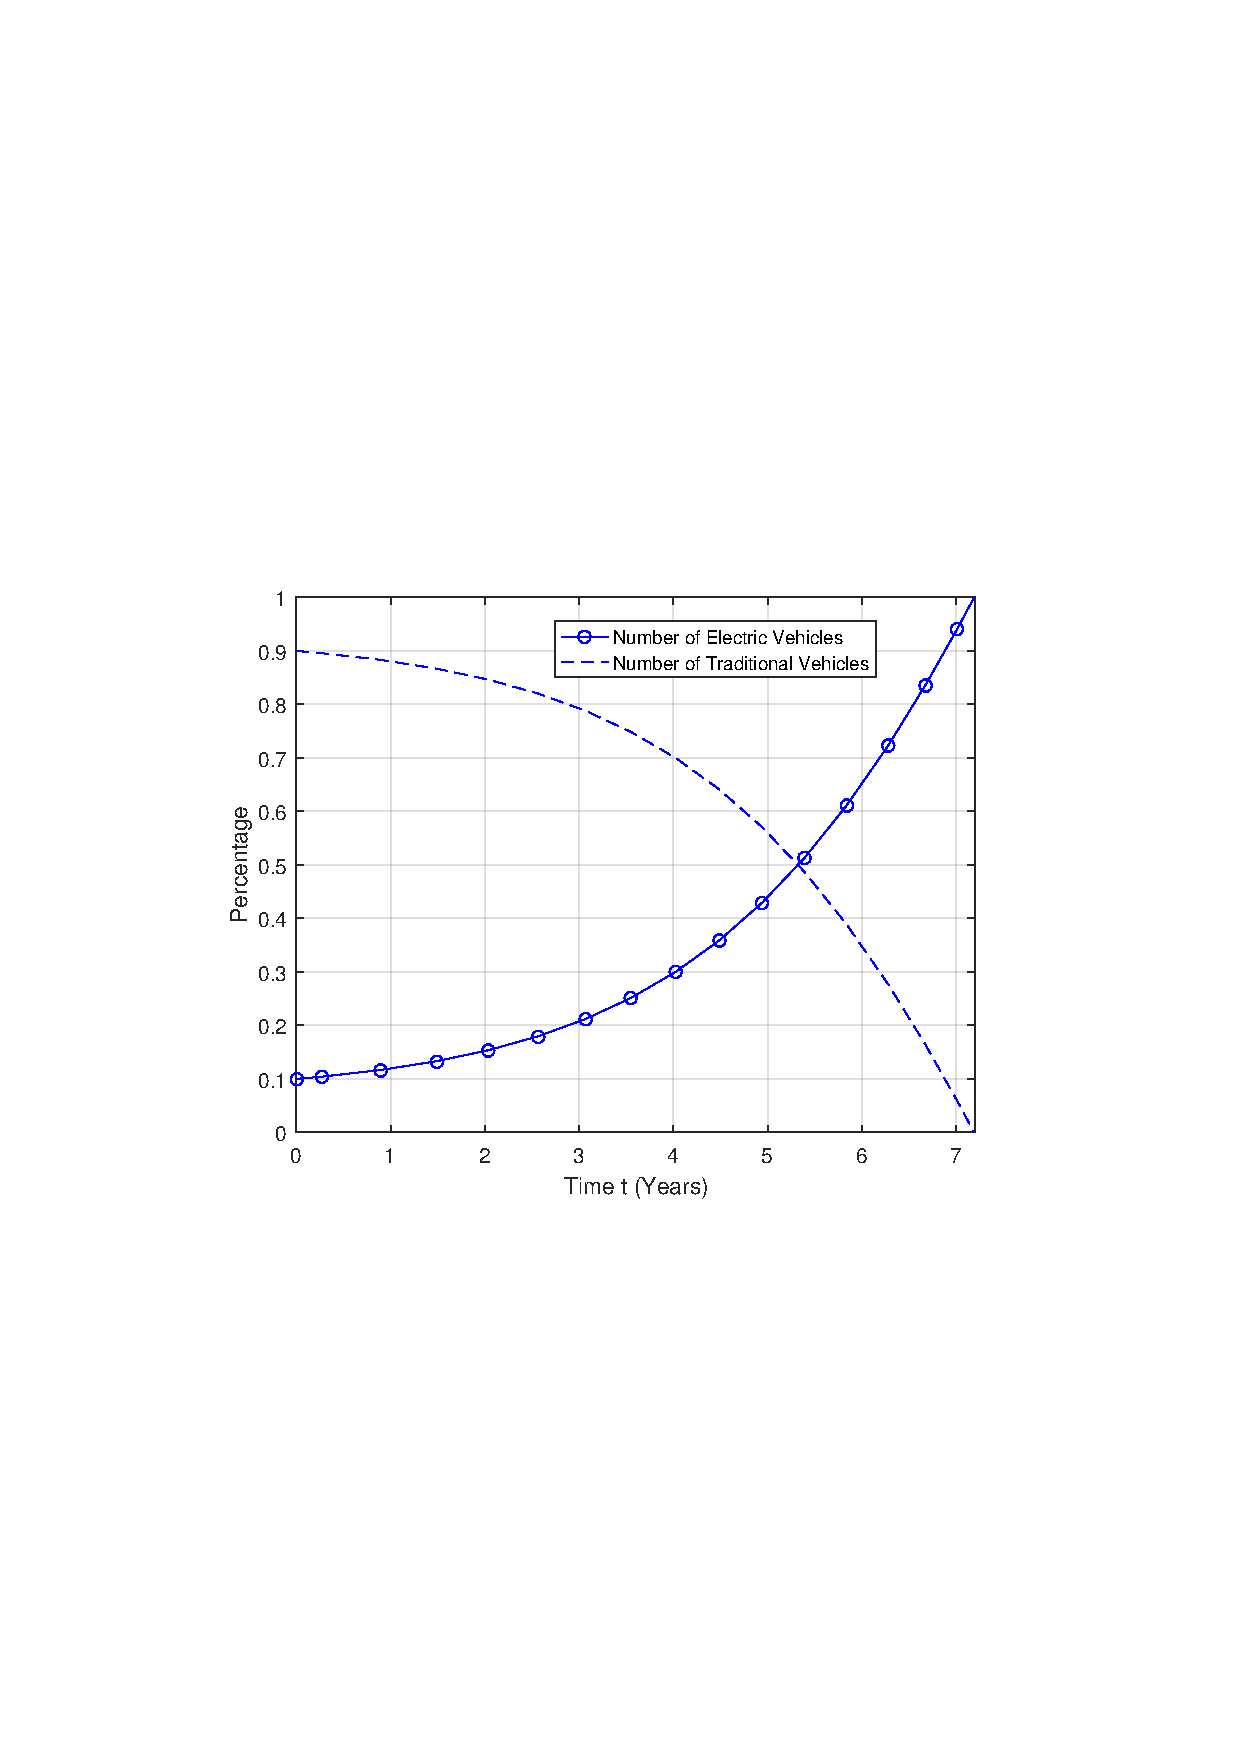
\includegraphics[width=3in]{evolution.pdf}
%\vspace{-0.1in}
\caption{The Evolution Process in Ireland}
\label{fig_evolution}
%\vspace{-0.2in}
\end{figure}
From Figure~\ref{fig_evolution},
we can see that $10\%$

\subsection{City-based Charger, Rural Charger, Population Density Distribution and Wealth Distribution}
\begin{figure}[h]
\centering
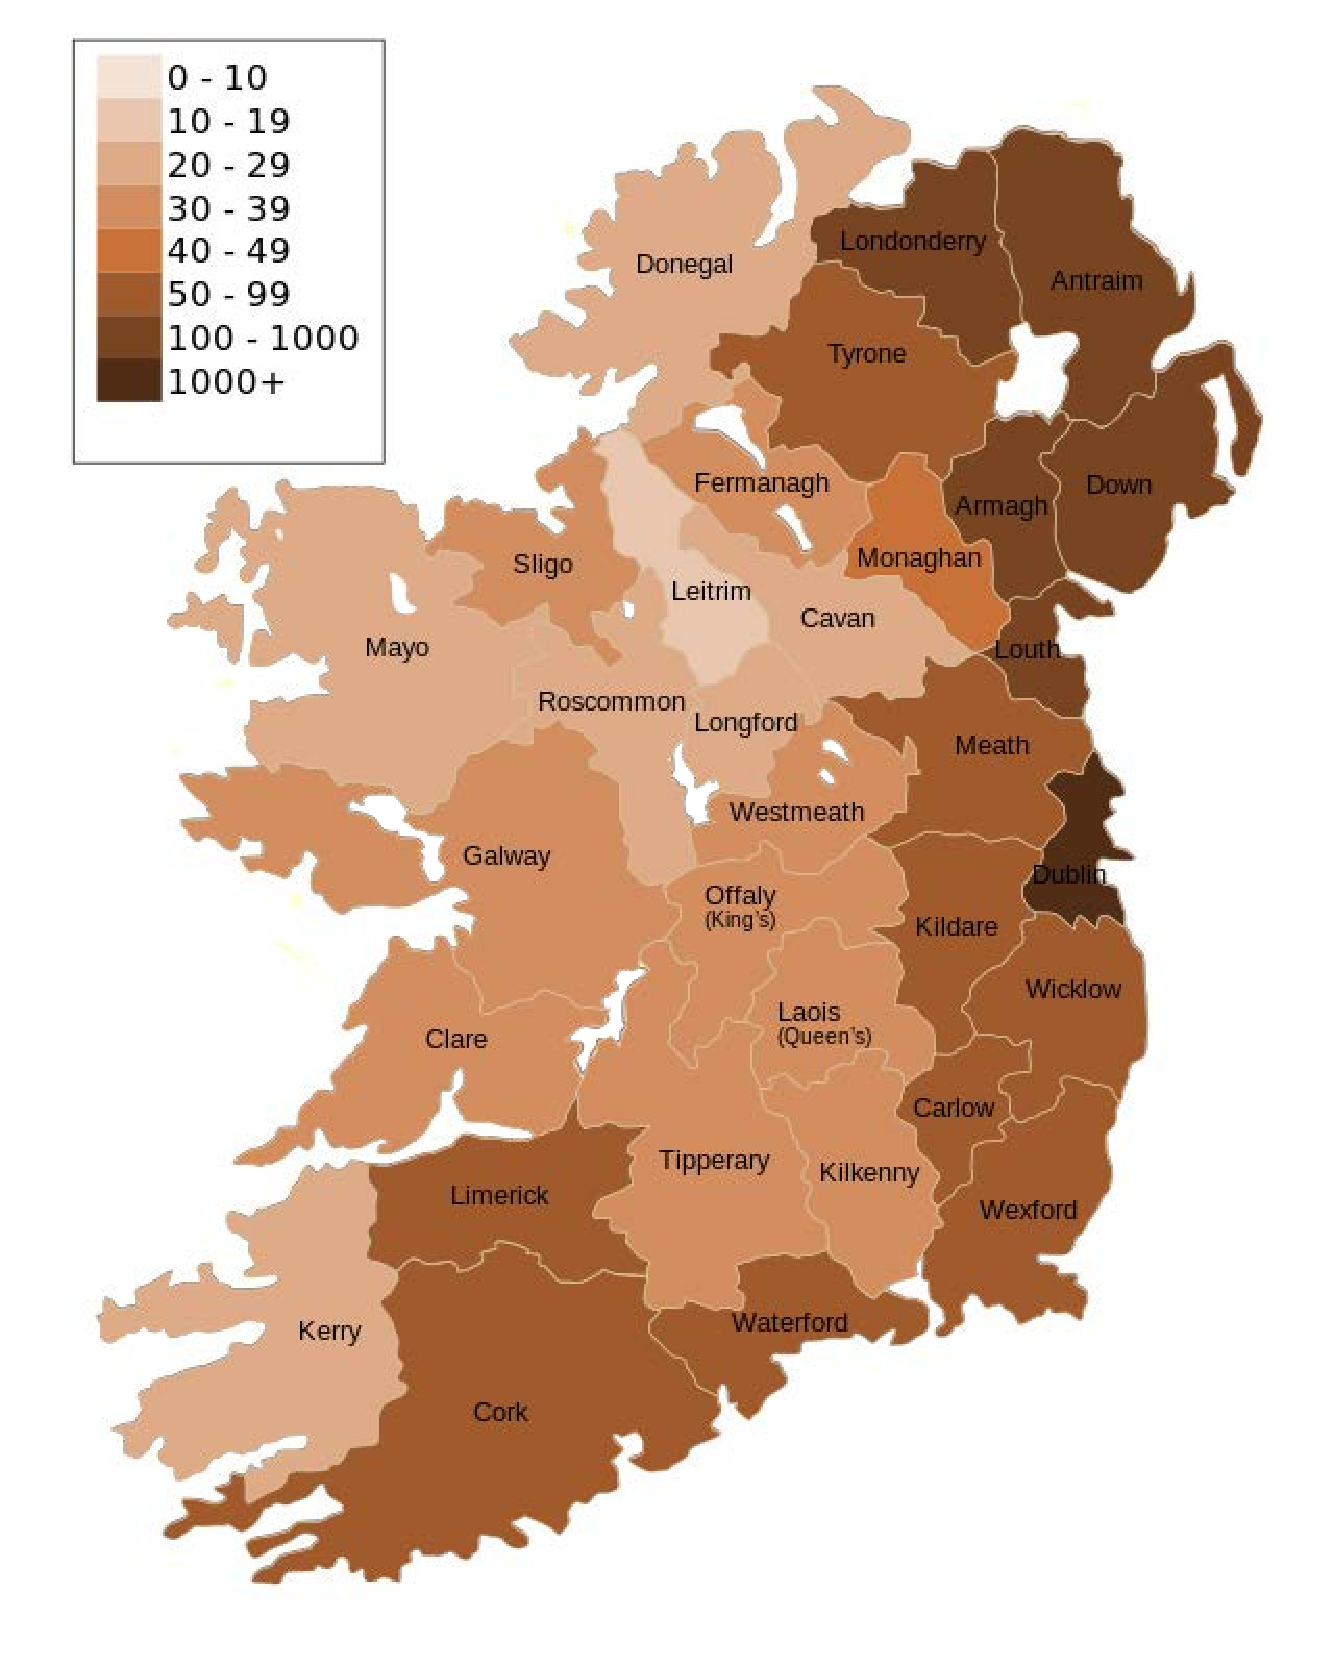
\includegraphics[width=2in]{Ire_Population_Dens.pdf}
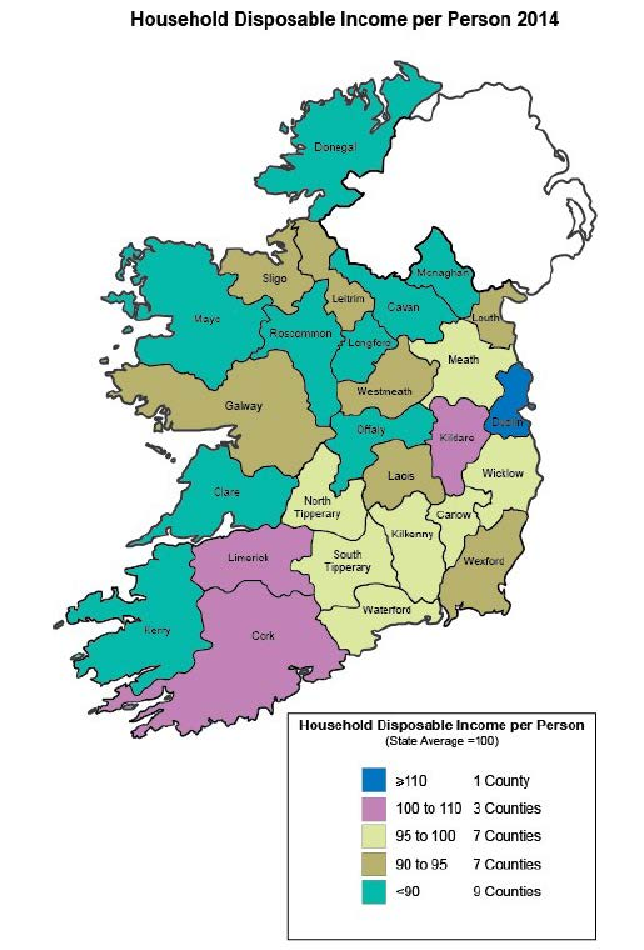
\includegraphics[width=2in]{Ire_wealth.pdf}
%\vspace{-0.1in}
\caption{Interstate difference of Ireland.}
\label{fig_stages_Populatoin}
%\vspace{-0.2in}
\end{figure}



As shown in Figure~\ref{fig_stages} the first stage is the current distribution of charging stations in Ireland.
The algorithm automatically generates the distribution after five years and after a decade, which are stage 2 and 3 respectively.
It shows that the second stage covers most of the cities, villages and towns.
Which is not surprising since not only does the urban area have a higher population density it also has a higher income per capita.
It is also worthy noting that the interstate difference of population density as well as disposable income per household may also impact the time evolution process.

\subsection{Other Transportation Options}
With the development of car-sharing, ride-share services as well as the self-driving cars,
it can be predicted that the information exchanges between charging stations will be greatly increased.
This increasing demand of station-station interaction will consequently stimulates the development of data-sharing network.

The simultaneous data-sharing network system may further enhances the power of electric vehicles from several aspects:
It can both optimize the usage of electric charging station,
shorten the averaged-queueing time and help drivers of the electric vehicles to decide the most reasonable routes when they are traveling from one city to another.

The battery-swap stations may replace the superchargers among the highway since there is no doubt that changing the battery is much more convenient and less time-consuming comparing with stopping at the charging station and waiting for the vehicles to be charged.

Although flying cars and Hyperloops are still prototypes currently, we are quite confident that the rapid development of battery cell will boost the popularization of flying cars and Hyperloops. Noting that the energy consumptions of both flying cars and Hyperloops are relatively high, therefore the electric charing system has to be well planned and established to support these consumptions.
